\documentclass[12pt]{article}

% set margins and spacing
\addtolength{\textwidth}{1.3in}
\addtolength{\oddsidemargin}{-.65in} %left margin
\addtolength{\evensidemargin}{-.65in}
\setlength{\textheight}{9in}
\setlength{\topmargin}{-.5in}
\setlength{\headheight}{0.0in}
\setlength{\footskip}{.375in}
\renewcommand{\baselinestretch}{1.0}
\linespread{1.0}

% load miscellaneous packages
\usepackage{csquotes}
\usepackage[american]{babel}
\usepackage[usenames,dvipsnames]{color}
\usepackage{graphicx,amsbsy,amssymb, amsmath, amsthm, MnSymbol,bbding,times, verbatim,bm,pifont,pdfsync,setspace,natbib}

% enable hyperlinks and table of contents
\usepackage[pdftex,
bookmarks=true,
bookmarksnumbered=false,
pdfview=fitH,
bookmarksopen=true,hyperfootnotes=false]{hyperref}

% define environments
\newtheorem{definition}{Definition}
\newtheorem{fact}{Fact}
\newtheorem{result}{Result}
\newtheorem{proposition}{Proposition}



\begin{document}
\title{Crime and Drug Treatment across Detroit}
\author{Rachel Gaudreau\thanks{Syracuse University, Economics Department. Email: regaudre@syr.edu.} \and Sophia Oritz-Heaney\thanks{Syracuse University, Economics Department. Email} \and Weston Maechling\thanks{Syracuse University, Economics Department. Email: wrmaechl@syr.edu.} \and Leo Gershman\thanks{abc}}
\date{\vskip-.1in \today}
\maketitle

\vskip.3in
\begin{center} {\bf Abstract} \end{center}

\begin{quote}
{\small Insert abstract text here: 75-200 words, very high-level summary of your project.}
\end{quote}

\bigskip
\section{Introduction} \label{sec:introduction}

Answer the questions
\begin{enumerate}
    \item \textbf{Why should the reader care? / Why is the topic important?} (required)
    \item Why did you choose this topic? (optional)
    \item \textbf{What question will you answer? How will you do it?} (required)
        \begin{enumerate}
            \item If your theory/hypothesis fit in one paragraph, include it here. If it is longer, make it a separate section after the lit review. EITHER OPTION IS FINE as long as the length is sufficient/appropriate for your project.
        \end{enumerate}
    \item \textbf{What did you find?} (required)
    \item \textbf{Give a "road map" of the paper. Where will the reader find the various parts of your work?} (required)
\end{enumerate}

\section{Literature Review} \label{sec:literature}

Discuss at least five papers that are closely related to your results (more is better). Explain how they're related. Did you find something similar, or different? Did you look at a different context? Different time period? Different level of detail?

The geographical relationship between crime and access to mental health care is a widely studied topic but can be convoluted. For example, mental illness is associated with an increased likelihood of substance abuse, which directly and indirectly relates an increase in crime to mental illness. One viable method of treating mental illness is through office-based mental healthcare. Thus, evidence shows that increasing access to office-based mental health care by 10 mental health care provider offices in a county can lead to a 0. 4\% reduction in the county crime rate. \cite{mental_healthcare_and_crime}). An increase in access to mental health care also shows a connection to participation in government disability programs. This is largely because better access to mental health facilities increases the likelihood of proper diagnosis of serious mental illness which leads to access to programs such as Supplemental Security Income (SSI) and Social Security Disability Insurance (SS(D)I). \cite{mental_health_and_disability}. While access to disability insurance does not directly relate to crime this shows that increasing access to mental health care allows for more opportunities for support and better access to the social safety net. Furthermore, this effect is also evident when specifically considering access to substance abuse treatment (SAT) facilities. Evidence shows that increasing access to SAT facilities reduces violent crime due to the effectiveness in reducing crimes motivated by obtaining money to purchase drugs, reducing violence among those in the drug trade, and reducing drug usage which eases aggressive behavior due to drug abuse \cite{SAT_centers_and_crime}. However, a significant barrier to this effect could be the price of substance abuse treatment. In a study conducted between 2002 and 2003, the median willingness to pay for drug rehabilitation is shown to be below the average cost of treatment. Moreover, the cost of drug treatment is a significant indicator of self-reported probability of enrollment. \cite{cost_of_drug_treatment}. While it is likely that cost of treatment has changed in the subsequent decades, it is still important to acknowledge barriers to treatment when considering its affects on crime rates in an urban area, such as Detroit. This also contributes to evidence of a positive feedback loop between drug usage, crime, and standard of living in a given area. Higher levels of drug usage leads to higher crime rates in a given geographical area which corresponds to lower standards of living due to the addictive properties of drugs, the numbing of decision making caused by drug usage, and the relationship between areas with lower standards of living and a higher tendency for those who live within such an area to turn to drugs as a means for escape \cite{drugs_and_crime}. 

\section{Theoretical Analysis}
\label{sec:theory}
Optional--may include in intro if it's short.


\section{Data}
\label{sec:data}

\subsection{911 Calls in Detroit Area (Dataset 1)}

This data comes from the City of Detroit Open Data Portal's Police Serviced 911 Calls  \href{https://data.detroitmi.gov/datasets/detroitmi::police-serviced-911-calls/about}{911-Data}. It is generated by the Detroit Police Department's Crime Data Analytics when a call is placed. This data set covers 911 calls that are received by precincts around the Detroit metropolitan area from the year 2016-2022. We isolated the observations to one year, 2017, from the original dataset 911-Data so we could perform cross-sectional analysis. This dataset is referred to as 2017-911-Calls. We chose observations from 2017 since the year a) overlaps with dataset 2 and b) is before COVID-19, where crime rates statistics shifted in general \cite{covid_and_crime}. This is to eliminate COVID-19 effects from affecting our data analysis. We used the longitude and latitude variables from 2017-911-Calls for cross-sectional-analysis with treatment-center dataset.

\subsection{Substance Abuse Treatment Centers (SATC) in Detroit Area (Dataset 2)}

This data is from the Substance Abuse and Mental Health Services Administration (SAMHSA). Data is generated through the National Survey of Substance Abuse Treatment Services \href{https://www.samhsa.gov/data/data-we-collect/n-ssats-national-survey-substance-abuse-treatment-services}{N-SSATS} an annual survey of all known public and private substance abuse treatment services in the United States. SAMHSA conducts this survey annually. This data covers the names and addresses of substance abuse treatment services in operation in the Detroit Metropolitan area between the years 2015 to 2021. 

\subsection{ArcGISPro}
We used the ArcGISPro application to layer both 2017 datasets and geocode their locations. Using the coordinates (longitude and latitude variables) of each point, we created two new variables:
\begin{itemize}
    \item near\textunderscore\ fid: This assigned every 911 call with one SATC, the center geographically closest to it. Variable is a numeric integer, with values ranging from 1 to 44. 
    \item near \textunderscore\ dist: This is the distance in meters the 911 call observation is from the SATC it is associated with in near\textunderscore\ fid. 
\end{itemize}
Since every 911 call (observation) is associated with only one SATC, no 911 call is counted twice. This is
\textit{If an observation of near \textunderscore\ dist is "-1", then that observation is} 

\subsection{Data Manipulation}
\begin{enumerate}
    \item Download raw datasets of "\href{https://data.detroitmi.gov/datasets/detroitmi::police-serviced-911-calls/about}{911 Calls}"and "\href{https://github.com/ecn310/course-project-zipcentercrime/blob/main/detroit_samhsa_sud_2015_2021.dta}{SATC} ". Make sure both datasets are saved as ".csv" files. (comma delimited)
    \item Open Stata/MP 18.0 and import the raw datasets. Follow this do file to isolate the observations to 2017.
\subsubsection{ArcGIS}
    \item Upload these datasets into ArcGISPro and create XY tables for both datasets. Follow this replication file here "\href{https://github.com/ecn310/course-project-zipcentercrime/blob/main/ArcGIS_Reproducability.md}{ArcGISPro Reproducibility File} "
    \item Use the "near" tool in ArcGISPro to create two new variables, near\textunderscore\ fid and near \textunderscore\ dist. It will add these columns/observations to the 911 calls dataset. 
    \item Export this updated dataset as a csv file. 
    \subsubsection{Stata}
    \item Open that dataset into Stata and follow this do file \href{C:\Users\sorti\OneDrive\Desktop\ArcDataDo.do.txt}{ArcData Do File}
    \item Create distance rings per distance (in meters) radius of the treatment center. The distance rings/parameters should be 50, 100, 250, 500, 750, 1000, 1250, 1500, 1750. These will become new observations in the dataset. 
    \item Perform a two-sample t-test on each coinciding parameter to identify if there is a statistical difference in the distribution of observations for each. 
\end{enumerate}

\subsection{Summary Statistics}
 summarize

    Variable |        Obs        Mean    Std. dev.       Min        Max
-------------+---------------------------------------------------------
    near_fid |         44        22.5    12.84523          1         44
dist_gro~_50 |         44    28.84091    66.19771          0        376
dist_gro~100 |         44    60.34091    77.67582          0        326
dist_gr~_250 |         44    308.4318    314.5254          0       1434
dist_gr~_500 |         44    989.8409    1014.308          0       4174
-------------+---------------------------------------------------------
dist_gr~_750 |         44    1049.955    698.9852          0       2645
dist_gr~1000 |         44    1346.773    943.0601          0       3742
dist_gr~1250 |         44    1455.886    1202.573          0       5552
dist_gr~1500 |         44    1217.795    1222.337          0       5014
dist_gr~1750 |         44    1054.182    1104.161          0       4129
-------------+---------------------------------------------------------
dist_gr~2000 |         44    731.1591    824.6483          0       2816
ratio dist_group_100/dist_group_50

Ratio estimation                            Number of obs = 44

     _ratio_1: dist_group_100/dist_group_50

--------------------------------------------------------------
             |             Linearized
             |      Ratio   std. err.     [95% conf. interval]
-------------+------------------------------------------------
    _ratio_1 |   2.092199   .8721967      .3332463    3.851151
--------------------------------------------------------------

Ratio estimation                            Number of obs = 44

     _ratio_1: dist_group_250/dist_group_100

--------------------------------------------------------------
             |             Linearized
             |      Ratio   std. err.     [95% conf. interval]
-------------+------------------------------------------------
    _ratio_1 |   5.111488   1.337423      2.414317    7.808659
--------------------------------------------------------------

. ratio dist_group_50/dist_group_100

%Describe your data. Where you got it from, how it was generated, what variables you'll use, what data cleaning steps you had to take, where your processed data, code and documentation is stored.
%In a published paper, a lot of this detail will be in a data appendix. For the purposes of this report, include it all here (this may be the longest section of your report).

\section{Notes from 11/14/24:}
\begin{itemize}
    \item think about the opening and closing potentially
    \item Think about how to deal with the farther data points and potentially overlapping, sharing
    \item Only isolate 911 calls to specific drug related ones 
    \item doing zip code level with population density data and number of 911 calls in each density
    \item Only doing this in 2017 - specific we are only analyzing 2017, not just each year
    \end{itemize}
\subsection{Survey data}

\section{Results}
\label{sec:result}
%State your working hypothesis and null hypothesis - Explain why the statistics you’re presenting are appropriate -Present statistics and explain what they mean (e.g., do your results support the working hypothesis? 

%Explain what analyses you did, provide evidence (like in the descriptive stats exercise, but refined and clear) and then explain what your results mean.

For the research question on "How does the distance to the closest drug rehabilitation center relate to the amount of calls to 911?" our group hypothesized that as the distance from a drug treatment facility increases, the number of 911 calls also increases. This means that the further someone is from a treatment center, the more  likely that 911 would be called with a drug related inquiry. Our null hypothesis in this case would then be that there is no relation between distance to a drug treatment center and likelihood to call 911. 
\begin{figure}
    \centering
    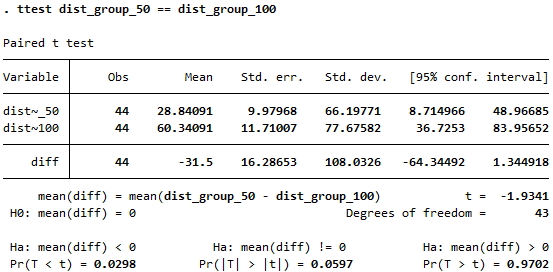
\includegraphics[width=1\linewidth]{image50-100.png}
        \caption{Paired t test showing the likelihood of a call coming from within 50 to 100 meters}
    \end{figure}
\begin{figure}
    \centering
    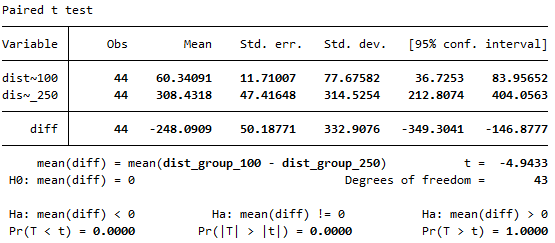
\includegraphics[width=1\linewidth]{image100-250.png}
    \caption{Paired t test showing the likelihood of a call coming from within 100 to 250 meters}
\end{figure}
\begin{figure}
    \centering
    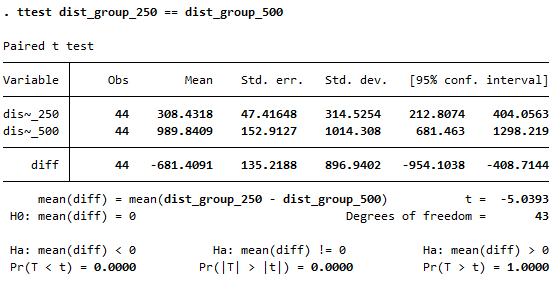
\includegraphics[width=1\linewidth]{image250-500.png}
    \caption{Paired t test showing the likelihood of a call coming from within 250 to 500 meters}
\end{figure}
\begin{figure}
    \centering
    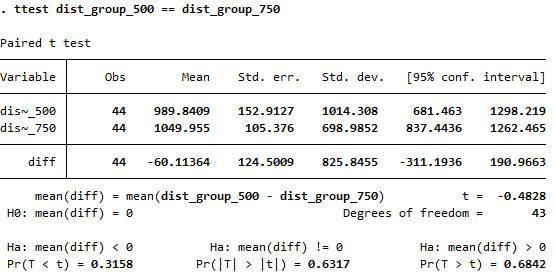
\includegraphics[width=1\linewidth]{image500-750.png}
    \caption{Paired t test showing the likelihood of a call coming from within 500 to 750 meters}
\end{figure}
\begin{figure}
    \centering
    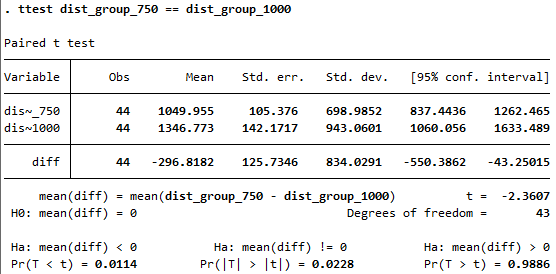
\includegraphics[width=1\linewidth]{image750-1000.png}
    \caption{Paired t test showing the likelihood of a call coming from within 750 to 1000 meters}
\end{figure}
\begin{figure}
    \centering
    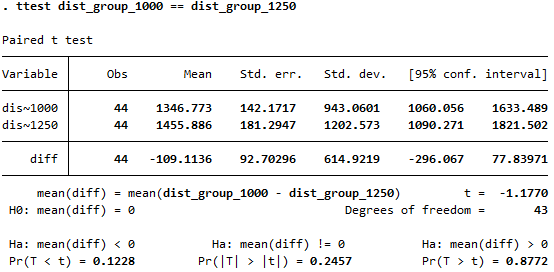
\includegraphics[width=1\linewidth]{image1000-1250.png}
    \caption{Paired t test showing the likelihood of a call coming from within 1000 to 1250 meters}
\end{figure}
\begin{figure}
    \centering
    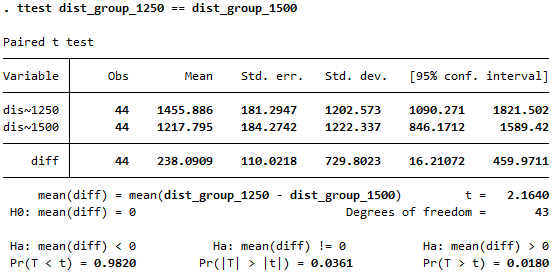
\includegraphics[width=1\linewidth]{image1250-1500.png}
    \caption{Paired t test showing the likelihood of a call coming from within 1250 to 1500 meters}
\end{figure}
\begin{figure}
    \centering
    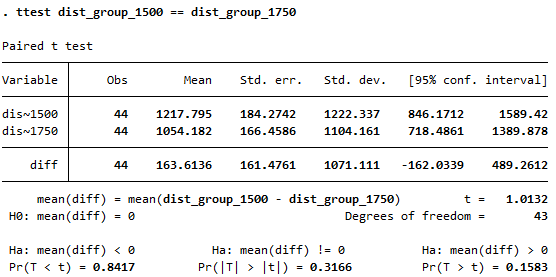
\includegraphics[width=1\linewidth]{image1500-1750.png}
    \caption{Paired t test showing the likelihood of a call coming from within 1500 to 1750 meters}
\end{figure}
\begin{figure}
    \centering
    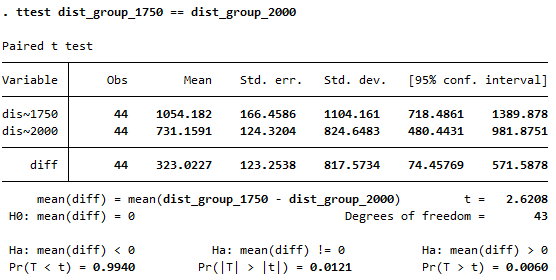
\includegraphics[width=1\linewidth]{image1750-2000.png}
    \caption{Paired t test showing the likelihood of a call coming from within 1750 to 2000 meters}
\end{figure}
   
Our current research show that the likelihood of a 911 call increases the closer someone is to a drug treatment center, at least within 1250 meters. The high confidence interval of these sections also helps to prove that there is a strong correlation between distance to a treatment center and likelihood of 911 call. In the future we plan on organizing this into a more detailed graph. Before then we also plan on cutting down on the amount of 911 calls used in the datasets by focusing only on those that are directly related to drug or violence related incidents. Along with that, our group hopes to show the correlation over time between new treatment centers and lowered 911 calls. Our original hypothesis was proven to be false, but we have ideas on why areas closer to treatment centers would have more calls.

Our first theory is that these treatment centers were placed in areas of high crime and low standards of living. These places would naturally have a higher rate of 911 calls. Along with that, some readings we looked at say that affluent communities petition against the construction of rehab centers near them to ensure people with those issues have no reason to be near them.

The second theory is that these treatment centers were built in densely populated areas. These areas would naturally have more people than their surroundings. These people would also call the police more often and have more issues.

Regardless of the reason, our research so far shows that the closer an area is to a drug or alcohol rehab center, the higher likelihood it is more 911 calls will come out of it. This leads into our discussion on the further implications of areas near these research centers being more dangerous.

\section{Discussion}
\label{sec:discussion}

Optional. This is where you would discuss any of the following
\begin{itemize}
    \item caveats (are there problems with the data that there are no obvious ways to resolve? if so, how might this impact
    \item future work / next steps
    \item implications of the results: that is, how your findings -- if they were causally identified -- might inform policymaking, etc.
\end{itemize}

\section{Conclusion}
\label{sec:conclusion}

Re-state (in different words) what you did and what you learned. If your discussion (Section 6) would be short, you can just have a Conclusion section that includes your discussion (that is, leave out a separate Discussion section).

\newpage
\section*{Bibliography}
\singlespacing
\setlength\bibsep{0pt}

\bibliographystyle{chicago}
\bibliography{reference.bib}


\newpage
\section*{Data Appendix} \label{sec:appendixa}
\addcontentsline{toc}{section}{Appendix A}

You should at least direct your reader to your replication package. You might put key elements of your replication package in this section as well.

\end{document}